\section{Multiple coordinate spaces}

Coordinate spaces are all over the place. In robotics a point cloud is defined in the space of its sensor. To make actual use of this data we transform the point cloud to be in the space of the robot itself. It is a requirement to be able to think in different coordinate spaces in order to do any serious work. Let's quickly take a look at some common coordinate spaces and how to transform between one coordinate space and another.

\subsection{Common coordinate spaces}

\subsubsection{Object space}

The object space describes vertices of some object to a shared origin. When artists create some model, e.g. a tank, they start modelling the various meshes around an origin within a modelling program like Blender. All the vertices of the various meshes of the model are saved to some file which can be loaded by a game engine.

\subsubsection{World space}

Any interesting game consists of various models each described in their own object space. However, to create a nice world every model gets placed at some world coordinate relative from each other. To properly display the created world all coordinates need to be transformed to this shared world.

\subsubsection{Upright space}

Upright space is a step between object and world space. In upright space the rotation of the world space is already applied. To go from upright space to world space only requires some translation. This space is not always used in tutorials or books, but it is a nice step to make it easier to reason about a switch between coordinate spaces.

\subsubsection{Camera space}

Camera space is the object space associated with the viewpoint used for rendering. The camera space determines which parts of the world are visible.

\subsection{Object space to world space}

Let's take a brief look at an example of transforming a simple pyramid from object space to some world space. First, of all let's define the vertices of the pyramid.

\begin{itemize}
	\item Top: $\begin{bmatrix}
		0 & 2 & 0
	\end{bmatrix}^\intercal$
	\item Front left: $\begin{bmatrix}
		-2 & 0 & -2
	\end{bmatrix}^\intercal$
	\item Front right: $\begin{bmatrix}
		2 & 0 & -2
	\end{bmatrix}^\intercal$
	\item Back left: $\begin{bmatrix}
		-2 & 0 & 2
	\end{bmatrix}^\intercal$
	\item Back right: $\begin{bmatrix}
		2 & 0 & 2
	\end{bmatrix}^\intercal$
\end{itemize}

Furthermore, we know that the world position to be $\begin{bmatrix}2 & 0 & 3\end{bmatrix}^\intercal$, the used coordinate system is left handed and the pyramid is rotated $45^\circ$. With this information we can also state the basis vectors relative to the world space.

\begin{itemize}
	\item Position: $\begin{bmatrix}2 & 0 & 3\end{bmatrix}^\intercal$
	\item $\textbf{p}=\begin{bmatrix}0.707 & 0 & 0.707\end{bmatrix}^\intercal$
	\item $\textbf{q}=\begin{bmatrix}0 & 1 & 0\end{bmatrix}^\intercal$
	\item $\textbf{r}=\begin{bmatrix}0.707 & 0 & -0.707\end{bmatrix}^\intercal$
\end{itemize}

$\textbf{p}$, $\textbf{q}$ and $\textbf{r}$ is a common notation to denote the basis vectors. Basis vectors specify how to interpret coordinates within its space. Good basis vector are orthonormal, that is all vectors are perpendicular to each other and of unit length. Read the book for the exact reasons why. Yup, I choose the easy way out. Now onto the fun part: converting object coordinates to world space!

To transform the vertices of the pyramid to world space we need to apply its basis vectors. Basis vector can contain various transformation like scaling, reflection and rotation. More about these in the chapter about matrices. In this case we only store the rotation relative to the world space. Once the basis vectors are applied all vertices are defined in terms of \textit{upright space}. All that is left to do is to translate all vertices by the position the pyramid is assigned within world space. After this final step all vertices are defined in terms of world space. Note that upright space is not necessary to define explicitly, but it makes it easier to reason about the transformation.

\subsubsection{Transforming a single vertex}

As an example let's transform the front left vertex ($\begin{bmatrix}
		-2 & 0 & -2
	\end{bmatrix}^\intercal$) from object space to world space. Thus we need to apply the basis vectors to the vertex:

$$\textbf{u}=-2\begin{bmatrix}0.707 \\ 0 \\ 0.707\end{bmatrix}+0+-2\begin{bmatrix}0.707 \\ 0 \\ -0.707\end{bmatrix}=\begin{bmatrix}-2.828 \\ 0 \\ 0\end{bmatrix}$$

As stated in the previous chapter the dot product is able to determine how much of a vector goes into a specific direction. This is exactly why we apply the basis vectors against the $x$, $y$, and $z$ coordinate. Now that the axes are aligned there is one final step remaining: we have to add the world position the the upright coordinate:

$$\textbf{w}=\begin{bmatrix}-2.828 \\ 0 \\ 0\end{bmatrix}+\begin{bmatrix}2 \\ 0 \\ 3\end{bmatrix}=\begin{bmatrix}-0.828 \\ 0 \\ 3\end{bmatrix}$$

\subsubsection{Transforming the pyramid}

Let's visualize the pyramid transformation to get a better feel for these coordinate spaces. The values for each of the coordinates are specified in table \ref{tab:pyramid-coordinates-transformation}. In figure \ref{fig:pyramid-object-space} we show the pyramid in its own object space. We specified that we want to rotate our pyramid by $45^\circ$, so we expect to see a rotated pyramid in upright space (figure \ref{fig:pyramid-upright-space}). Finally, to go from upright space to world space the rotation should not just, but only a translation should be applied. This is exactly what happens in figure \ref{fig:pyramid-world-space}. So at this point mess around with the formulas a bit. Convert coordinates between the various spaces and try to understand the diagrams.

\begin{table}[H]
\centering
\begin{tabular}{|l|l|l|l|}
\hline
\textbf{Position} & \textbf{Object space} & \textbf{Upright space} & \textbf{World space} \\ \hline
Top & $\begin{bmatrix}0 & 2 & 0\end{bmatrix}^\intercal$ & $\begin{bmatrix}0 & 2 & 0\end{bmatrix}^\intercal$ & $\begin{bmatrix}2 & 2 & 3\end{bmatrix}^\intercal$ \\ \hline
Front left & $\begin{bmatrix}-2 & 0 & -2\end{bmatrix}^\intercal$ & $\begin{bmatrix}-2.828 & 0 & 0\end{bmatrix}^\intercal$ & $\begin{bmatrix}-0.828 & 0 & 3\end{bmatrix}^\intercal$ \\ \hline
Front right & $\begin{bmatrix}2 & 0 & -2\end{bmatrix}^\intercal$ & $\begin{bmatrix}0 & 0 & 2.828\end{bmatrix}^\intercal$ & $\begin{bmatrix}2 & 0 & 5.828\end{bmatrix}^\intercal$ \\ \hline
Back left & $\begin{bmatrix}-2 & 0 & 2\end{bmatrix}^\intercal$ & $\begin{bmatrix}0 & 0 & -2.828\end{bmatrix}^\intercal$ & $\begin{bmatrix}2 & 0 & 0.172\end{bmatrix}^\intercal$ \\ \hline
Back right & $\begin{bmatrix}2 & 0 & 2\end{bmatrix}^\intercal$ & $\begin{bmatrix}2.828 & 0 & 0\end{bmatrix}^\intercal$ & $\begin{bmatrix}4.828 & 0 & 3\end{bmatrix}^\intercal$ \\ \hline
\end{tabular}
\caption{Pyramid coordinates transformation}
\label{tab:pyramid-coordinates-transformation}
\end{table}

\begin{figure}[H]
\centering
    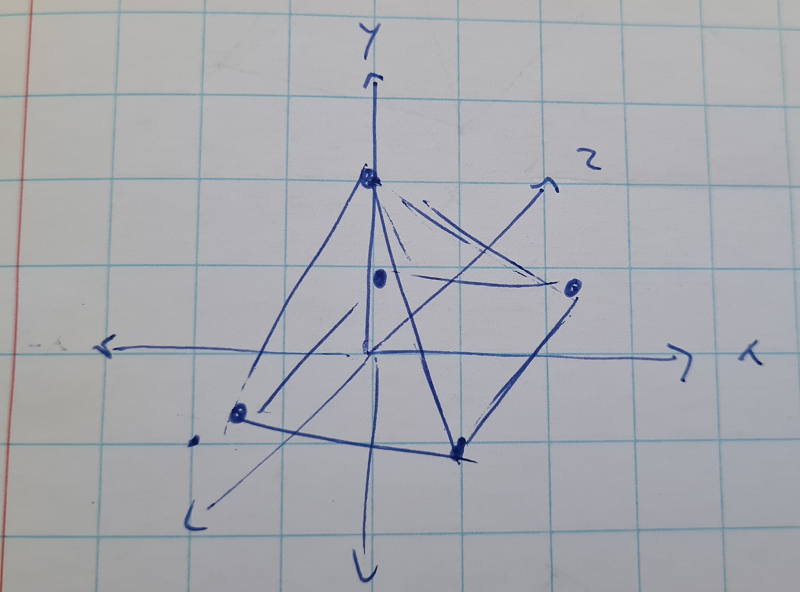
\includegraphics[scale=0.65]{03_object_space}
\caption{Pyramid in object space}
\label{fig:pyramid-object-space}
\end{figure}

\begin{figure}[H]
\centering
    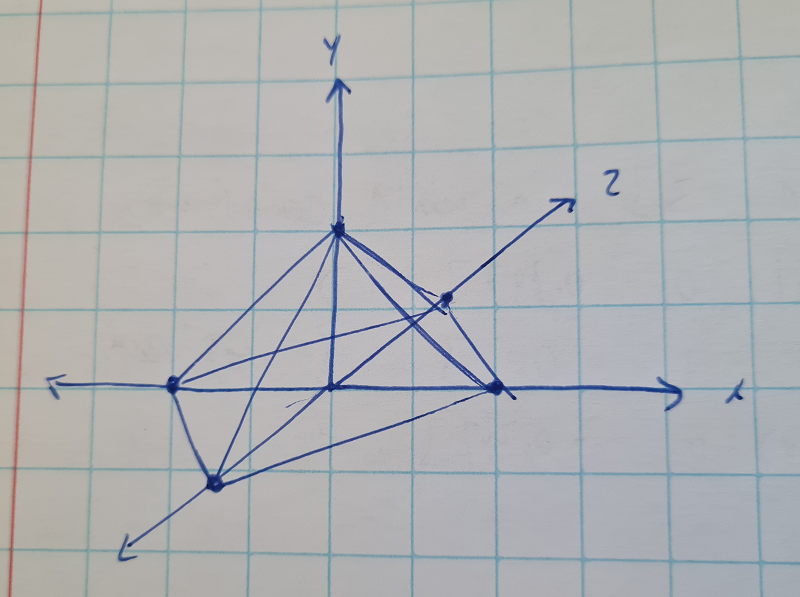
\includegraphics[scale=0.65]{03_upright_space}
\caption{Pyramid in upright space}
\label{fig:pyramid-upright-space}
\end{figure}

\begin{figure}[H]
\centering
    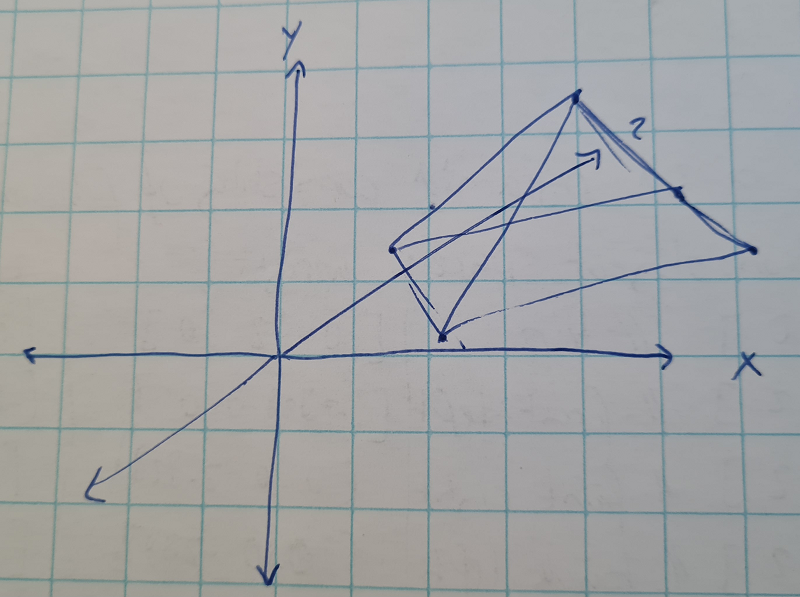
\includegraphics[scale=0.65]{03_world_space}
\caption{Pyramid in world space}
\label{fig:pyramid-world-space}
\end{figure}

\subsubsection{General formulas}

Let $\textbf{v}$ be an arbitrary vertex is object space, $\textbf{u}$ equal to $\textbf{v}$ transformed in upright space and $\textbf{w}$ equal to $\textbf{v}$ transformed in world space. Furthermore, the basis vectors $\textbf{p}$, $\textbf{q}$ and $\textbf{r}$ with world position $\textbf{o}$.

$$\textbf{u}=v_x\textbf{p}+v_y\textbf{q}+v_z\textbf{r}$$

$$\textbf{w}=\textbf{o}+\textbf{u}=\textbf{o}+v_x\textbf{p}+v_y\textbf{q}+v_z\textbf{r}$$

\subsection{Object space to world space}

To go from world space to object space we need to reverse the process described in the previous section. The formulas to achieve this are as follows:

$$\textbf{u}=\textbf{w}-\textbf{o}$$

$$\textbf{v}=\begin{bmatrix}
\textbf{u}\cdot\textbf{p} \\ \textbf{u}\cdot\textbf{q} \\ \textbf{u}\cdot\textbf{r}
\end{bmatrix}$$
